\chapter{Softwarearchitektur}
Durch die Klasse \textit{SceneManager} wird die Aufbaulogik gesetzt und auch die Reihenfolge, was passiert wenn die entsprechende Szene geladen wird oder wenn diese Szene jetzt erst mal nicht mehr angezeigt werden soll. Im weiterem werden dort auch sehr Elementare Spielregeln gesetzt. Das \textit{Model} hält alle wichtigen Daten, welche für den Spielverlauf wichtig sind. Die \textit{ViewModels} halten die explizierte Logik für jede Szene und die Elementaren Spielregeln der jeweiligen Szene.
 

\section{Model}

\begin{figure}[H]
	\centering
	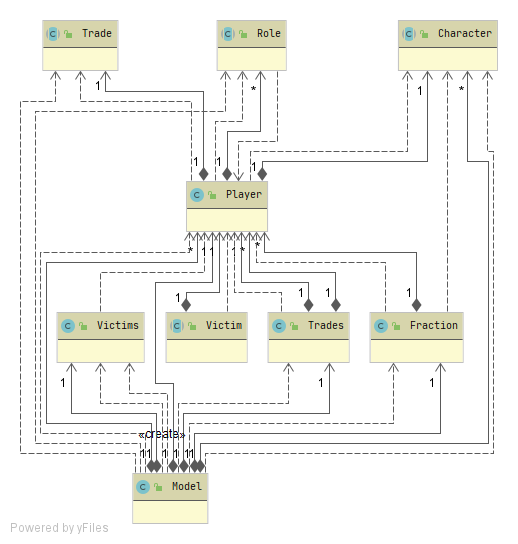
\includegraphics[width=0.8\textwidth]{architektur/model_uml.png}
	\caption{Übersicht Model}
	\label{figure:diagram_model}
\end{figure}

In Abbildung \ref{figure:diagram_model} ist eine grobe Übersicht über das Model zu sehen. Die Hauptklasse des Models ist die Klasse \textit{Model}. Die Klasse \textit{Player} speichert alle relevanten Informationen über einen Spieler ab. Jedem Spieler kann ein Charakter (\textit{Character}), sowie ein Beruf (\textit{Trade}) zugeordnet sein. Für Aktionen des Spielers können ihm mehrere Rollen (\textit{Role}) zugeordnet sein. Die Klasse \textit{Fraction} speichert die Fraktionen der Spieler. Die Klasse \textit{Trades} speichert die Spieler anhand ihres Berufes. Die Klasse \textit{Victims} speichert die Opfer der einzelnen Charaktere. Jede dieser Klassen befindet sich jeweils in einem gleichnamigen Package.

\medskip
Die Klassen \textit{Character}, \textit{Role}, \textit{Trade} und \textit{Victim} sind abstrakt, um für die unterschiedlichen Implementierungen der verschiedenen Charaktere, Rollen, Berufe und Opfer eine einheitliche Ansprache zu gewährleisten, indem diese hiervon abgeleitet werden. Die Klassen \textit{Fraction} und \textit{Trades} sind als Singletons realisiert.

\medskip
In den folgenden Unterkapiteln werden die einzelnen Packages des Models betrachtet. 

\subsection{Model (Package)}
Die Klasse \textit{Model} ist die Hauptklasse des Models. Innerhalb dieses Unterkapitels wird im Folgenden mit Model jeweils die Klasse und nicht das gesamte Model bezeichnet. 
Hier werden die allgemeinen Daten für eine Spielrunde abgespeichert. Außerdem erfolgt hierüber der Zugriff auf einige weitere Objekte, die beispielsweise die Opfer oder die Fraktionen verwalten. 

Es werden zunächst die Attribute des Models betrachtet.

\medskip
\begin{center}
	\begin{minipage}{0.7\textwidth}
		\lstinputlisting[firstnumber=19, firstline=19, lastline=36, caption=Model Attribute (1), label= lst:modelAttribute01]{../src/main/java/de/werwolf_spielleiter/model/Model.java}
	\end{minipage}
\end{center}


In \autoref{lst:modelAttribute01} sind die Attribute zu sehen, die Anzahlen abspeichern. Das Attribut \textit{countPlayer} speichert die Anzahl der Mitspieler. Die weiteren Attribute speichern jeweils die Anzahl der jeweiligen Charaktere. Das Attribut \textit{countWerewolf} speichert beispielsweise die Anzahl der Werwölfe. 

\medskip
\begin{center}
	\begin{minipage}{0.7\textwidth}
		\lstinputlisting[firstnumber=38, firstline=38, lastline=48, caption=Model Attribute (2), label= lst:modelAttribute02]{../src/main/java/de/werwolf_spielleiter/model/Model.java}
	\end{minipage}
\end{center}

In \autoref{lst:modelAttribute02} sind zunächst die Attribute des Hauptmanns zu sehen. Das Attribut \textit{sheriff} speichert ab, ob mit Hauptmann gespielt wird. Die Attribute \textit{sheriffWasVote} und \textit{nextSheriffVote} speichern ab, ob bereits ein Hauptmann gewählt wurde, bzw. ob ein Nachfolger als Hauptmann bestimmt werden muss. 
Das Attribut \textit{hunterPhase} speichert ab, ob der Jäger sich ein Opfer suchen muss. 
Das Attribut \textit{greatWolfInfected} speichert ab, ob der Urwolf bereits ein Werwolf Opfer infiziert hat. 
Das Attribut \textit{werewolfDead} speichert ab, ob bereits ein Werwolf* \footnote{Werwolf in beliebiger Gestalt: einfacher Werwolf, Urwolf, Großer, böser Wolf, Weißer Werwolf, Wildes Kind als Wolf, Wolfshund als Wolf, infiziertes Werwolf Opfer} getötet wurde. 

\medskip
\begin{center}
	\begin{minipage}{0.7\textwidth}
		\lstinputlisting[firstnumber=50, firstline=50, lastline=55, caption=Model Attribute (3), label= lst:modelAttribute03]{../src/main/java/de/werwolf_spielleiter/model/Model.java}
	\end{minipage}
\end{center}

In \autoref{lst:modelAttribute03} sind die Attribute bezüglich der Berufe zu sehen. 
Das Attribut \textit{playWithTrade} speichert ab, ob mit Berufen gespielt wird. Die drei nachfolgenden Attribute speichern die jeweilige Anzahl der verschiedenen Berufe. Das Attribut \textit{countVagabond} speichert beispielsweise die Anzahl der Vagabunden. Das Attribut \textit{allowConfession} gibt zu jedem Zeitpunkt Auskunft darüber, ob der Beichtvater gerade seine Aktion ausführen darf. 

\medskip
\begin{center}
	\begin{minipage}{0.7\textwidth}
		\lstinputlisting[firstnumber=57, firstline=57, lastline=67, caption=Model Attribute (4), label= lst:modelAttribute04]{../src/main/java/de/werwolf_spielleiter/model/Model.java}
	\end{minipage}
\end{center}

Die ersten beiden Attribute in \autoref{lst:modelAttribute04} speichern jeweils die Liste aller Spieler, bzw. die Liste aller lebenden Spieler. 
Das Attribut \textit{cardThiefList} speichert die beiden Charaktere für den Dieb. 
Das Attribut \textit{night} speichert ab, ob gerade Tag oder Nacht ist. Ist es \textit{false}, ist gerade Tag. 
Das Attribut \textit{day} speichert die Anzahl der Tage, die seit Beginn der Spielrunde verstrichen sind. Begonnen wird mit der Zählung bei eins. 

\medskip
\begin{center}
	\begin{minipage}{0.7\textwidth}
		\lstinputlisting[firstnumber=69, firstline=69, lastline=79, caption=Model Attribute (5), label= lst:modelAttribute05]{../src/main/java/de/werwolf_spielleiter/model/Model.java}
	\end{minipage}
\end{center}

In Abbildung \autoref{lst:modelAttribute05} sind zunächst einige weitere Objekte gespeichert, die Teile des Spiels verwalten. Das Attribut \textit{fraction} speichert die Referenz auf das Objekt, das die Fraktionen der Spieler verwaltet. 
Das Attribut \textit{trades} speichert die Referenz auf das Objekt, das die Berufe der Spieler verwaltet. 
Das Attribut \textit{victims} speichert die Referenz auf das Objekt, das die Opfer der Charaktere verwaltet. 
Das Attribut \textit{idolWildChild} speichert die Referenz auf den Spieler, der das Vorbild des Wilden Kindes ist. 

\begin{figure}[H]
	\centering
	\includegraphics[width=0.75\textwidth]{architektur/model_methods.pdf}
	\caption{Model Methoden}
	\label{figure:model_methods}
\end{figure}

In Abbildung \ref{figure:model_methods} sind die Methoden des Models dargestellt. Die \textit{get} und \textit{set} Methoden, sowie Methoden um die \textit{boolean} Attribute abzufragen oder zu setzen, wurden hier der Übersichtlichkeit wegen nicht aufgeführt. Zu fast jeder Variable gibt es solche Methoden.

\medskip
Die Methode \textit{resetModel(): void} setzt das Model für eine neue Spielrunde zurück. \\
Die Methode \textit{getCharsStack(): List<Character>} liefert anhand der gespeicherten Anzahlen der Charaktere eine Liste mit Charakter Objekten. In dieser Liste kommt jeder Charakter anhand seiner gespeicherten Anzahl vor.

\medskip
Die Methode \textit{startGame(): void} startet eine Spielrunde. Zunächst werden alle Spieler zur Liste der lebenden Spieler hinzugefügt. Es wird die Methode \textit{getCharsStack()} aufgerufen, um eine Liste mit Charakteren zu bekommen.
Anschließend wird jedem Spieler aus dieser Liste zufällig ein Charakter zugeteilt. Dazu bekommt er die entsprechenden Rollen. Außerdem wird er seiner Fraktion (passend zur Charakterkarte) zugeordnet. 
Wird mit Berufen gespielt, wird danach jedem Spieler zufällig ein Beruf zugeteilt. 
Ist einem der Spieler der Dieb als Charakter zugeteilt worden, werden abschließend die zwei Charaktere für den Dieb zufällig aus der anfangs erhaltenen Liste mit Charakteren ausgewählt. 

\medskip
Die Methode \textit{getTradeStack(): List<Trade>} liefert anhand der gespeicherten Anzahlen der Berufe eine Liste mit Trade Objekten. In dieser Liste kommt jeder Beruf anhand seiner gespeicherten Anzahl vor. 

\medskip
Die Methode \textit{startNight(): void} startet die Nacht. Die Variable für die Nacht (\textit{night}) wird auf \textit{true} gesetzt. Die Variable für die Tage (\textit{dax}) wird inkrementiert. Abschließend wird das \textit{Victims} Objekt zurückgesetzt. 

\medskip
Die Methode \textit{initPlayerList(size: int): void} setzt die Spieleranzahl (\textit{countPlayer}) auf die übergebene Anzahl. Außerdem wird die Liste aller Spieler als leere Liste initialisiert, falls sie das noch nicht ist. 

\medskip
Die Methode \textit{isRoleInGame(role: Role): boolean} prüft, ob ein lebender Spieler die übergebene Rolle hat. Ist das der Fall, wird \textit{true} zurückgegeben, andernfalls \textit{false}. 

\medskip
Die Methode \textit{getFirstPlayerWithRole(role: Role): Player} gibt den ersten Spieler aus der Liste der lebenden Spieler zurück, der die übergebene Rolle hat. Hat kein Spieler diese Rolle, wird \textit{null} zurückgegeben. 

\medskip
Die Methode \textit{addPlayer(player: Player): boolean} fügt den übergebenen Spieler der Liste aller Spieler hinzu, wenn die Referenz nicht \textit{null} ist. Im letzteren Fall ist der Rückgabewert \textit{false}, andernfalls \textit{true}. 

\medskip
Die Methode \textit{die(player: Player): boolean} lässt einen übergebenen Spieler sterben, wenn die Referenz nicht \textit{null} ist. Dabei wird der Spieler aus der Liste der lebenden Spieler entfernt. Außerdem wird das \textit{Fraction} Objekt angewiesen, den Spieler zu entfernen, sowie der Spieler aus dem \textit{Trades} Objekt entfernt. War der Spieler ein Werwolf, wird gespeichert, dass bereits ein Werwolf gestorben ist. Abschließend wird der Spieler angewiesen, sich selbst sterben zu lassen. Ist der übergebene Spieler \textit{null}, ist der Rückgabewert \textit{false}, andernfalls ist er \textit{true}. 

\medskip
Die Methode \textit{changeThiefToNewCharacter(player: Player, newCharacter: Character): boolean} setzt dem Dieb (\textit{player}) den übergebenen Charakter (\textit{newCharacter}) als neuen Charakter. 
Dabei wird der Dieb zunächst aus dem \textit{Fraction} Objekt entfernt. Danach wird ihm der neue Charakter, sowie die zugehörigen Rollen gesetzt. Abschließend wird er wieder dem \textit{Fraction} Objekt hinzugefügt und dabei automatisch der richtigen Fraktion zugeordnet. Ist eine der übergebenen Referenzen \textit{null}, ist der Rückgabewert \textit{false}, andernfalls ist er \textit{true}.  

\subsection{Player}

Die Klasse \textit{Player} repräsentiert einen Spieler innerhalb einer Spielrunde. Dafür existieren folgende Attribute: 

\medskip
\begin{center}
	\begin{minipage}{0.7\textwidth}
		\lstinputlisting[firstnumber=21, firstline=21, lastline=29, caption=Player Attribute, label= lst:playerAttribute]{../src/main/java/de/werwolf_spielleiter/player/Player.java}
	\end{minipage}
\end{center}

Das Attribut \textit{name} speichert den Namen des Spielers. 
Das Attribut \textit{status} speichert den Status des Spielers. Dies kann beispielsweise \textit{alive} oder \textit{dead} sein. 
Das Attribut \textit{characterCardBack} speichert die Rückseite der Charakterkarte. 
Das Attribut \textit{characterCardFront} speichert die Vorderseite der Characterkarte. 
Das Attribut \textit{characterCardProperty} speichert die aktuell angezeigte Seite der Characterkarte. 
Das Attribut \textit{awake} speichert, ob der Spieler gerade aufgewacht ist, oder schläft. Wichtig ist dieses Attribut nur nachts, da tagsüber eh alle Spieler wach sind. 
Das Attribut \textit{character} speichert den Charakter, den der Spieler in der Spielrunde verkörpert. 
Das Attribut \textit{rolesList} speichert alle Rollen des Spielers. 
Das Attribut \textit{trade} speichert den Beruf des Spielers. Hat er keinen, ist dieses Attribut \textit{null}. 

\medskip
\begin{figure}
	\centering
	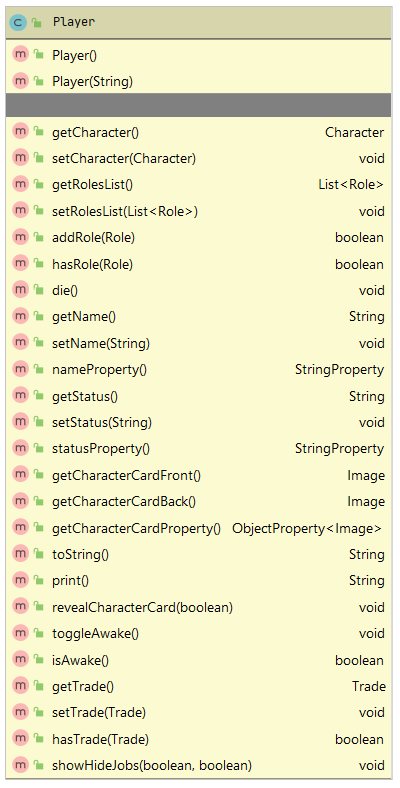
\includegraphics[width=9cm]{architektur/player_methods.png}
	\caption{Player Methoden}
	\label{figure:player_methods}
\end{figure}

Wie in \autoref{figure:player_methods} zu sehen, besitzt Player zwei Konstruktoren. Zunächst einen Konstruktor ohne Variablen. Dieser ist dazu da, den Spieler schon einmal anzulegen, ohne dass der Nutzer bereits einen Namen eingegeben haben muss. Der zweite bekommt einen String übergeben. Dies ist der Name des anzulegenden Spielers. 

\medskip
Weiterhin stehen diverse \textit{get} und \textit{set} Methoden zur Verfügung, um den Spieler zu manipulieren. 

\medskip
Die Methode \textit{addRole(role: Role): boolean} fügt dem Spieler die übergebene Rolle hinzu, falls er die Rolle noch nicht hat. In diesem Fall ist der Rückgabewert \textit{true}. Hat der Spieler die Rolle bereits, wird sie nicht noch einmal hinzugefügt und der Rückgabewert ist \textit{false}. 

\medskip
Die Methode \textit{hasRole(r: Role): boolean} gibt Aufschluss darüber, ob der Spieler die übergebene Rolle besitzt. In dem Fall ist der Rückgabewert \textit{true}. Besitzt er die Rolle nicht, ist der Rückgabewert \textit{false}. 

\medskip
Die Methode \textit{die(): void} lässt den Spieler sterben. Dazu setzt sie den Status auf \textit{dead}. 

\medskip
Die Methode \textit{toString(): String} gibt den Namen des Spielers zurück. 

\medskip
Die Methode \textit{print(): String} liefert eine etwas ausführlichere String Representation als \textit{toString()}. 

\medskip
Die Methode \textit{revealCharacterCard(reveal: boolean): void} setzt die aktuell angezeigte Seite der Charakterkarte. Ist der übergebene Wert \textit{true}, so wird die Vorderseite gesetzt, andernfalls die Rückseite. 

\medskip
Die Methode \textit{toggleAwake(): void} invertiert den Erwachenszustand. 

\medskip
Die Methode \textit{hasTrade(trade: Trade): boolean} gibt Aufschluss darüber, ob der Spieler den übergebenen Beruf hat. In dem Fall ist der Rückgabewert \textit{true}. Hat er den Beruf nicht, ist der Rückgabewert \textit{false}. 

\medskip
Die Methode \textit{showHideJobs(jobsRevealed: boolean, cardsRevealed: boolean): void} setzt das Bild der Charakterkarte entsprechend den beiden übergebenen Werte für den aktuellen Soll-Zustand der Karten. Ist \textit{jobsRevealed} \textit{true}, so wird das Berufsicon gesetzt. Ist \textit{jobsRevealed} \textit{false}, so wird die Vorderseite der Charakterkarte gesetzt, wenn \textit{cardsRevealed} \textit{true} ist. Andernfalls wird die Rückseite der Charakterkarte gesetzt. 

\subsection{Character}

\begin{figure}[H]
	\centering
	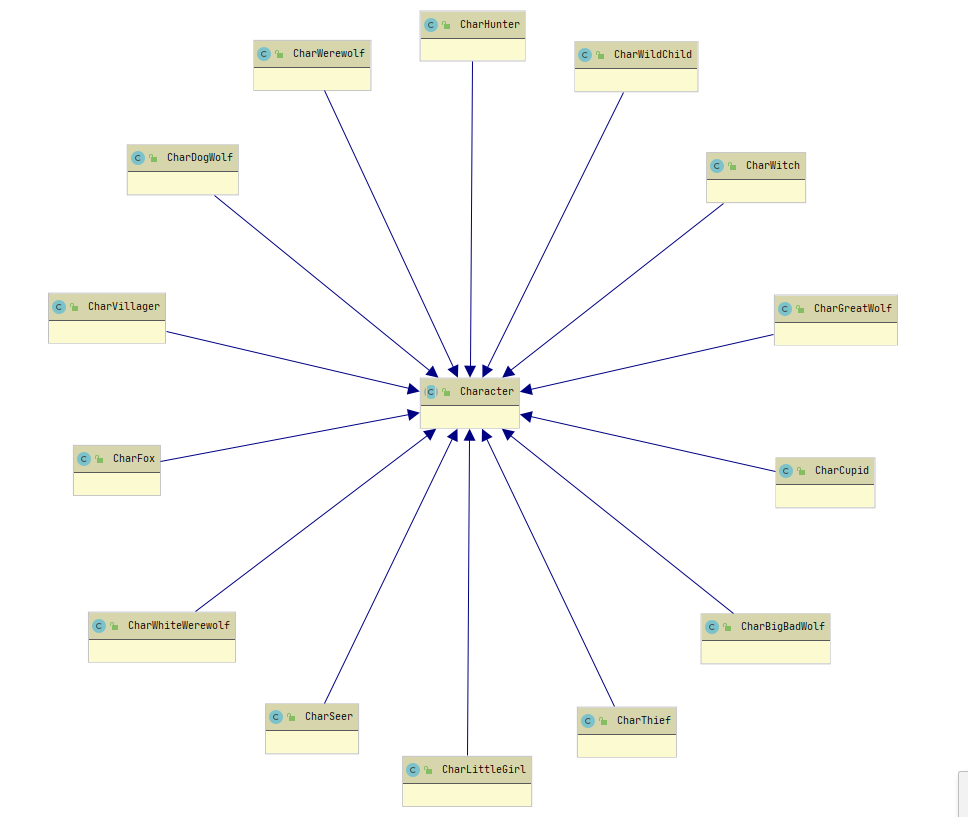
\includegraphics[width=14cm]{architektur/character_uebersicht.png}
	\caption{Character Übersicht}
	\label{figure:character_uebersicht}
\end{figure}

Alle Charaktere sind von der abstrakten Klasse \textit{Character} abgeleitet, wie in \autoref{figure:character_uebersicht} zu sehen. So ist für jeden Charakter eine einheitliche Ansprache gewährleistet und es können einfach weitere Charaktere implementiert werden. 

\medskip
\begin{center}
	\begin{minipage}{0.7\textwidth}
		\lstinputlisting[firstnumber=10, firstline=10, lastline=12, caption=Player Attribute, label= lst:characterAttribute]{../src/main/java/de/werwolf_spielleiter/character/Character.java}
	\end{minipage}
\end{center}

Wie in \autoref{lst:characterAttribute} zu sehen, hat die Klasse \textit{Character} drei Attribute. Das Attribut \textit{name} speichert den Namen des Charakters. Die Attribute \textit{characterCardBack} und \textit{characterCardFront} speichern die Rück- bzw. Vorderseite der zugehörigen Charakterkarte. 

\begin{figure}[H]
	\centering
	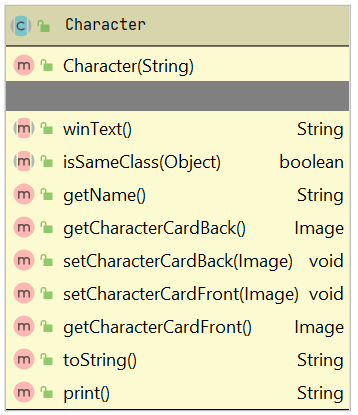
\includegraphics[width=6cm]{architektur/character_methods.png}
	\caption{Character Methoden}
	\label{figure:character_methods}
\end{figure}

Wie in \autoref{figure:character_methods} zu sehen, hat die Klasse \textit{Character} einen Konstruktor. Diesem wird der Name des Charakters übergeben. 

\medskip
Weiterhin gibt es als Schnittstelle für eingangs erwähnte Variablen \textit{get} und \textit{set} Methoden. 

\medskip
Die Methode \textit{toString(): String} liefert eine String Repräsentation des Charakters, die nur den Namen enthält. 
Die Methode \textit{print(): String} liefert eine etwas ausführlichere Repräsentation. 

\medskip
Die Methoden \textit{winText(): String} und \textit{isSameClass(obj Object): boolean} sind abstrakt. Diese werden von den abgeleiteten Klassen unterschiedlich implementiert. 

\medskip
Die meisten Charaktere unterscheiden sich nur in der Implementierung der vorgegebenen abstrakten Methoden und dem Konstruktor. Im Folgenden wird daher beispielhaft ein Charakter vorgestellt und die Unterschiede zu den anderen Charakteren dargelegt. 

\medskip
Die meisten Charaktere haben keine eigenen Attribute, diejenigen mit eigenen Attributen werden später betrachtet. 

\begin{figure}[H]
	\centering
	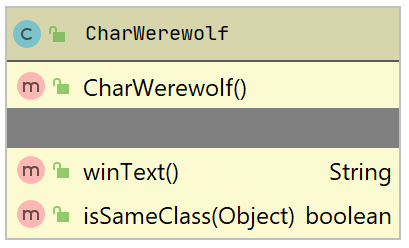
\includegraphics[width=6cm]{architektur/characterWerewolf_methods.png}
	\caption{Charakter Werwolf Methoden}
	\label{figure:characterWerewolf_methods}
\end{figure}

Wie in \autoref{figure:characterWerewolf_methods} zu sehen, wird exemplarisch die Klasse \textit{CharWerwolf} betrachtet. 
Wie erwähnt, erbt die se Klasse von \textit{Character} und hat keine eigenen Attribute. 

\medskip
Der Konstruktor ruft zunächst den Konstruktor von \textit{Character} mit dem Namen des Charakters auf. Anschließend werden die Vorder- und Rückseiten der Charakterkarte gesetzt. 

\medskip
Die Methode \textit{winText(): String} gibt den Text zurück, der angezeigt wird, wenn die Fraktion dieses Charakters gewinnt. 

\medskip
Die Methode \textit{isSameClass(obj: Object): boolean} gibt \textit{true} zurück, wenn das übergebene Objekt eine Instanz der selben Klasse ist, wie der Charakter, folglich also, wenn es derselbe Charakter ist. Andernfalls ist der Rückgabewert \textit{false}. 

\begin{figure}[H]
	\centering
	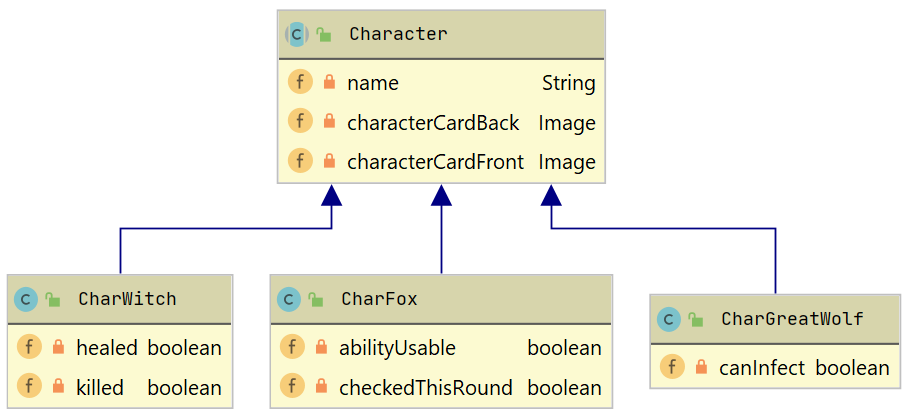
\includegraphics[width=11cm]{architektur/character_extra_attributes.png}
	\caption{Charaktere mit weiteren Attributen}
	\label{figure:character_extra_attributes}
\end{figure}

Wie in \autoref{figure:character_extra_attributes} zu sehen ist, gibt es drei Klassen, die weitere Attribute definiert haben. 

\medskip
Die Klasse \textit{CharWitch} hat die Attribute \textit{healed} und \textit{killed} um jeweils zu speichern, ob der Heiltrank, bzw. der Gifttrank in der Spielrunde schon eingesetzt wurde. Im Fall, dass er eingesetzt wurde, ist der Wert \textit{true}. 

\medskip
Die Klasse \textit{CharFox} hat das Attribut \textit{abilityUsable}, um zu speichern, ob der Fuchs seine Fähigkeit noch nutzen kann. Das Attribut \textit{checkedThisRound} speichert, ob der Fuchs in der aktuellen Nacht schon jemanden überprüft hat. 

\medskip
Die Klasse \textit{CharGreatWolf} hat das Attribut \textit{canInfect}, das speichert, ob der Urwolf noch jemanden infizieren kann. 

\begin{figure}[H]
	\centering
	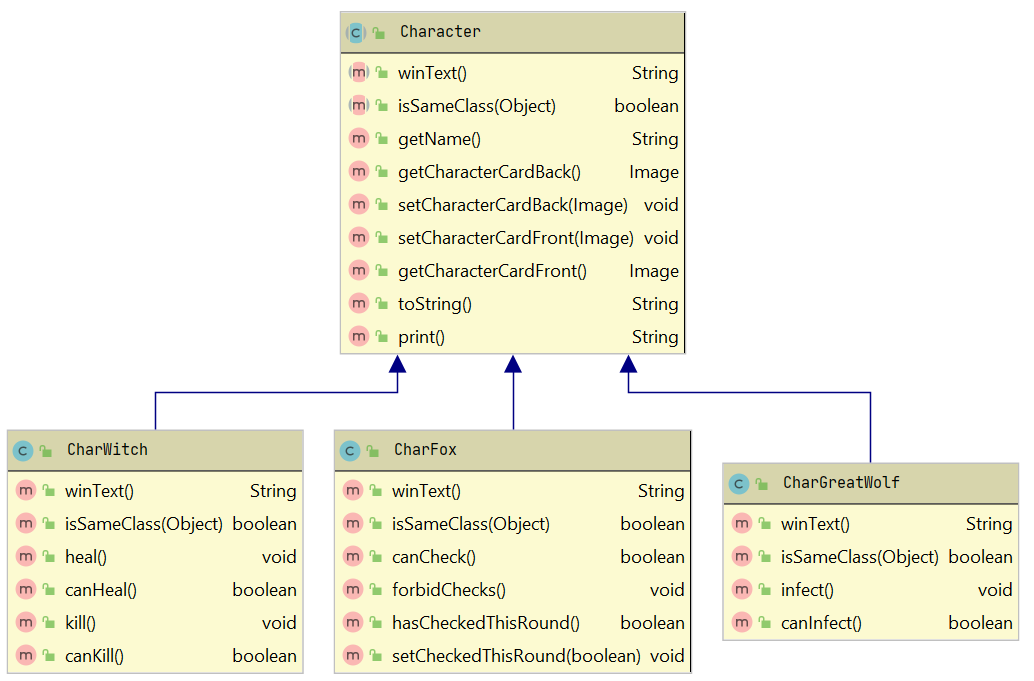
\includegraphics[width=13cm]{architektur/character_extra_methods.png}
	\caption{Charaktere mit weiteren Methoden}
	\label{figure:character_extra_methods}
\end{figure} 

Wie in \autoref{figure:character_extra_methods} zu sehen, haben die drei Klassen \textit{CharWitch}, \textit{CharFox} und \textit{CharGreatWolf} auch weitere Methoden definiert. 

\medskip
In der Klasse \textit{CharWitch} gibt es die Methode \textit{heal(): void} um zu speichern, dass die Hexe den Heiltrank eingesetzt hat. Die Methode \textit{canHeal(): boolean} gibt Auskunft darüber, ob die Hexe den Heiltrank schon eingesetzt hat. 
Die Methode \textit{canKill(): boolean} gibt Auskunft darüber, ob die Hexe den Gifttrank schon eingesetzt hat. 
Die Methode \textit{kill(): void} speichert ab, dass die Hexe den Gifttrank eingesetzt hat. 

In der Klasse \textit{CharFox} gibt es vier weitere Methoden. 
Die Methode \textit{canCheck(): boolean} gibt Aufschluss darüber, ob der Fuchs noch seine Fähigkeit besitzt. 
Die Methode \textit{forbidChecks(): void} entzieht dem Fuchs seine Fähigkeit. 
Die Methode \textit{hasCheckedThisRound(): boolean} gibt Aufschluss darüber, ob der Fuchs in der aktuellen Nacht bereits jemanden überprüft hat. 
Die Methode \textit{setCheckedThisRound(checkedThisRound: boolean): void} setzt den Wert dafür, ob der Fuchs in der aktuellen Nacht bereits jemanden überprüft hat. Ist der übergebene Wert \textit{true}, so hat der Fuchs bereits jemanden überprüft, ist er \textit{false}, so hat der Fuchs in der aktuellen Nacht noch niemanden überprüft. 

\medskip
In der Klasse \textit{CharGreatWolf} gibt es zwei weitere Methoden. 
Die Methode \textit{canInfect(): boolean} gibt Aufschluss darüber, ob der Urwolf seine einmalige Fähigkeit, das Werwolf Opfer zu infizieren, noch besitzt. 
Die Methode \textit{infect(): void} speichert, dass der Urwolf seine einmalige Fähigkeit bereits eingesetzt hat. Damit wird ihm seine einmalige Fähigkeit entzogen. 

\subsection{Role}

\begin{figure}[H]
	\centering
	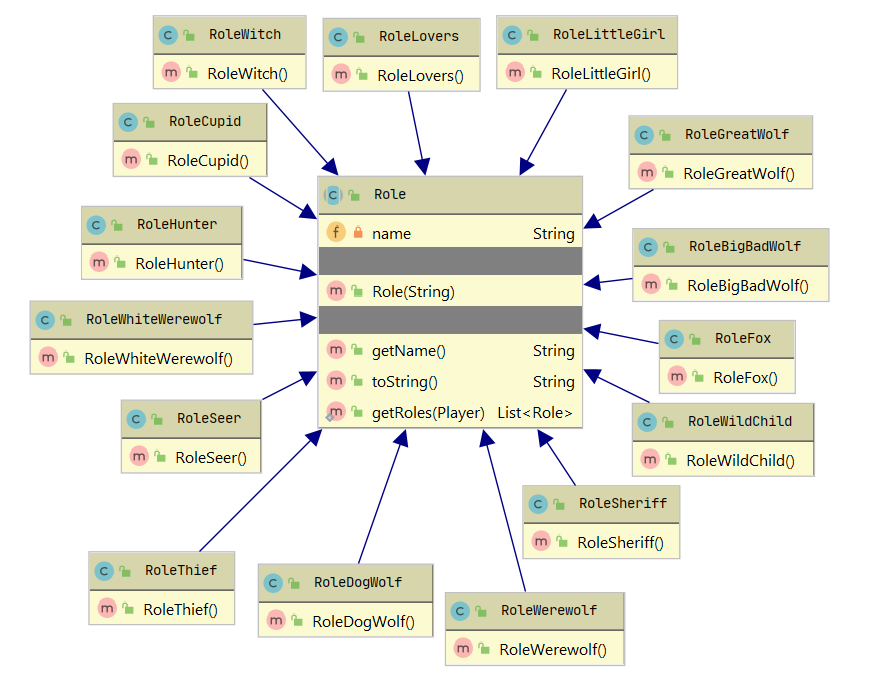
\includegraphics[width=\textwidth]{architektur/role_uml.png}
	\caption{Role Übersicht}
	\label{figure:role_uebersicht}
\end{figure}

Alle Rollen sind von der abstrakten Klasse \textit{Role} abgeleitet, wie in \autoref{figure:role_uebersicht} zu sehen. So ist für jede Rolle eine einheitliche Ansprache gewährleistet und es können einfach weitere Rollen implementiert werden. 

\medskip
Die Klasse \textit{Role} hat einen Konstruktor, der den Namen der Rolle als String übergeben bekommt. 
Der Name ist über die Methode \textit{getName(): String} zugänglich. 

\medskip
Mittels \textit{toString(): String} ist eine String Repräsentation der Rolle zugänglich, die den Namen enthält. 

\medskip
Die statische Methode \textit{getRoles(player: Player): List<Role>} gibt für einen übergebenen Spieler eine Liste mit den zu seinem Charakter gehörenden Rollen zurück. Hat der Spieler keinen Charakter gesetzt, wird eine leere Liste zurückgegeben. 

\medskip
Alle von \textit{Role} abgeleiteten Rollen haben nur einen Konstruktor, in dem der Konstruktor von \textit{Role} mit dem Namen der Rolle aufgerufen wird. 

\subsection{Fraction}

Die Klasse \textit{Fraction} ist als Singleton implementiert. 
Hier werden die Fraktionen, in denen die Spieler sind, verwaltet. 
Hier wird auch entschieden, ob eine Fraktion gewonnen hat und wenn ja, welche. 

\begin{figure}[H]
	\centering
	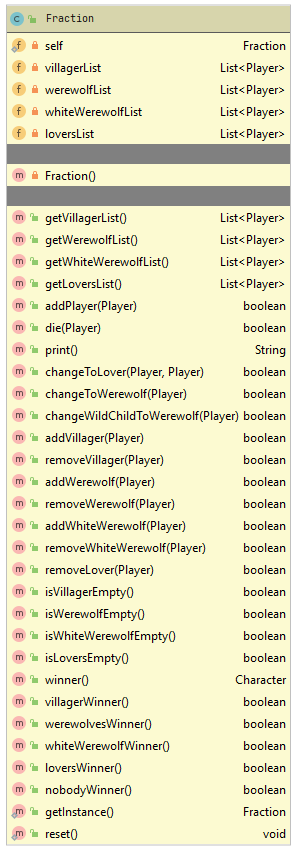
\includegraphics[width=0.45\textwidth]{architektur/fraction_uml.png}
	\caption{Fraction Übersicht}
	\label{figure:fraction_uebersicht}
\end{figure}

Wie in \autoref{figure:fraction_uebersicht} zu sehen besitzt die Klasse eine statische Klassenvariable, mit der Referenz auf das Singleton (\textit{self}). 
Weiterhin gibt es für die vier Fraktionen Dorfbewohner, Werwölfe, Weißer Werwolf und Liebespaar jeweils eine Liste mit den zugehörigen Spielern als Instanzvariable. 

\medskip
Für diese Listen gibt es jeweils eine \textit{get} Methode (z.B. \textit{getWerewolfList(): List<Player>}). 

\medskip
Es gibt sowohl eine Methode \textit{addPlayer(player: Player): boolean}, die einen übergebenen Spieler selbstständig zur richtigen Fraktion zuordnet, als auch für jede Fraktion eine eigene \textit{add} Methode (z.B. \textit{addWerewolf(player: Player): boolean}). Wenn jeweils keine Zuordnung zu einer Fraktion vorgenommen werden konnte, ist der Rückgabewert \textit{false}, im erfolgreichen Fall \textit{true}. Für jede Fraktion gibt es eine \textit{remove} Methode, um einen übergebenen Spieler aus der Fraktion zu entfernen. 

\medskip
Weiterhin gibt es für jede Fraktion eine Methode um zu prüfen, ob die jeweilige Fraktion keine Mitglieder enthält.

\medskip
Um zu testen, welche Fraktion gewonnen hat, gibt es zum Einen je Fraktion eine Methode, die prüft, ob die Fraktion gewonnen hat. Es gibt eine weitere Methode (\textit{winner(): Character}), die einen die Fraktion repräsentierenden Charakter zurückgibt, als Zeichen, welche Fraktion gewonnen hat. Ist hier der Rückgabewert \textit{null}, hat noch keiner gewonnen und das Spiel läuft noch. 

\medskip
Die Methode \textit{die(player: Player): boolean} entfernt einen übergebenen Spieler aus seiner Fraktion. 

\medskip
Mittels \textit{print(): String} lässt sich eine textuelle Repräsentation der Fraktionen generieren. 

\medskip
Mit der Methode \textit{changeToLover(player1: Player, player2: Player): boolean} lassen sich zwei Spieler zur Fratkion Liebespaar wechseln.
Die Methoden \textit{changetoWerewolf(player: Player): boolean} und \textit{changeWildChildToWerewolf(player: Player): boolean} wechseln einen beliebigen Spieler, bzw. das Wilde Kind, zur Fraktion der Werwölfe. 

\medskip
Um das Singleton zu erhalten, gibt es eine statische Methode \textit{getInstance(): Fraction}. 
Um das Singleton für eine neue Spielrunde zu reseten, gibt es die statische Methode \textit{reset(): void}. 

\subsection{Victim}

Das Package \textit{victim} enthält eine abstrakte Klasse \textit{Victim}, von der die einzelnen Opfer-Klassen erben. Außerdem befindet sich hier die Klasse \textit{Victims}, die die Opfer verwaltet und Zugriff auf sie gewährt. 

\medskip
\textit{Victims} hat je Opfer-Klasse eine Referenz auf dieses Opfer. 
Für jedes Opfer gibt es eine \textit{get} und eine \textit{set} Methode. 
Um abzufragen, ob es Nacht- oder Tagopfer gibt, gibt es die Methoden \textit{hasNightVictims(): boolean} bzw. \textit{hasLynchVictims(): boolean}. 
Abschließend gibt es eine Methode, um \textit{Victims} zu reseten (\textit{reset(): void}), sowie eine Methode \textit{print(): String}, um eine textuelle Repräsentation des Zustands von \textit{Victims} zu bekommen. 

\medskip
Die abstrakte Klasse \textit{Victim} speichert die Referenz auf einen Spieler, und die Todesursache als Text. 
Um diese abzufragen, existieren die Methoden \textit{getPlayer(): Player}, \textit{getDeathReason(): String} und \textit{isSet(): boolean}. Die letztgenannte Methode ist dazu da, um zu prüfen, ob das Opfer gesetzt wurde. Ansonsten ist der Rückgabewert bei \textit{getPlayer()} \textit{null}. 

\medskip
Jedes von \textit{Victim} abgeleitete Opfer hat zwei Konstruktoren, um das Objekt anzulegen und ein Attribut für die jeweilige Todesursache. Die eine Variante legt ein "leeres" Opfer an, die zweite eines mit Spieler und Todesursache. 
Einzig das Werwolf Opfer (\textit{VictimWerewolf}) hat noch weitere Methoden und Attribute. 
Hier gibt es noch Attribute, die speichern ob das Werwolf Opfer geheilt (\textit{healed}) oder infiziert (\textit{infected}) wurde. Dazu existieren Methoden diesen Zustand abzufragen, sowie um zu heilen, oder zu infizieren. 

\subsection{Trade}
\begin{figure}[H]
	\centering
	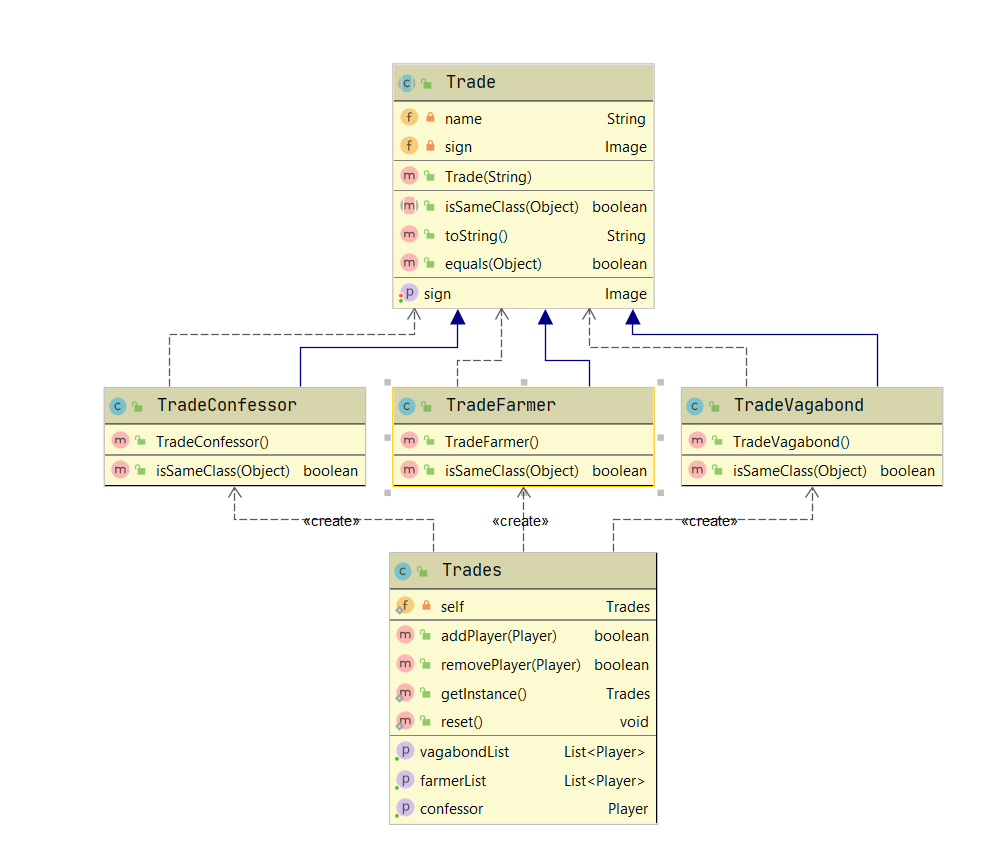
\includegraphics[width=\textwidth]{architektur/Trade_Uebersicht.png}
	\caption{Übersicht Trade (Package)}
	\label{figure:trade_uebersicht}
\end{figure}

Alle Berufe sind von der abstrakten Klasse \textit{Trade} abgeleitet, wie in \autoref{figure:trade_uebersicht} zu sehen ist. Dadurch ist für jeden Beruf eine einheitliche Ansprache gewährleistet und es können ohne weiteres neue Berufe implementiert werden.

\medskip
\textit{Trades} ist als Singleton implementiert, wo alle Informationen über die Spieler mit ihren Berufen gespeichert sind und somit im Spielverlauf auf bestimmte Berufe einzugehen, wenn sie eine bestimmtes Verhalten haben.
Die Methode \textit{reset()} setzt die Trades neu wenn ein neues Spiel gestartet wird.
\textit{addPlayer()} setzt die Spieler in die richtige Liste, welchen Beruf diese haben. Die Methode \textit{removePlayer()} wird aktiv, wenn ein Spieler im Spiel stirbt. Über die Methode \textit{getInstance()} kann man auf diezuvor genannten Methoden zugreifen.

\medskip
\textit{TradeConfessor}, \textit{TradeVagabond} und \textit{TradeFarmer} sind identisch aufgebaut, deshalb werden wir anhand der Klasse \textit{TradeFarmer} einmal erklären, wie die Methoden in den Klassen funktionieren.
In den jeweiligen Konstruktoren wird die Bezeichnung des Berufes gesetzt und auch sein Bild gesetzt, wo durch im Spiel ersichtlich ist, welcher Spieler welchen Beruf hat.
  
\section{View}

\begin{figure}[H]
	\centering
	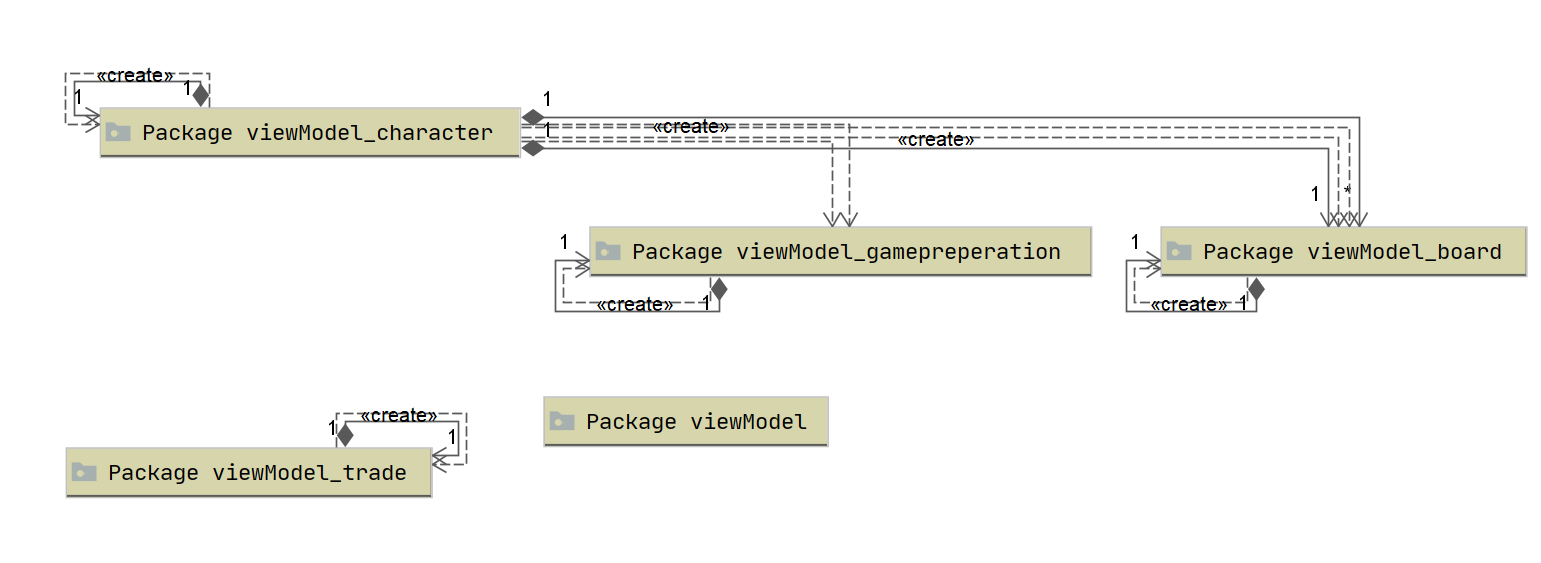
\includegraphics[width=\textwidth]{architektur/View_Packages_Uebersicht.png}
	\caption{Übersicht View}
	\label{figure:view_package_uebersicht}
\end{figure}

Die \autoref{figure:view_package_uebersicht} gibt einen Übersicht über die kompletten Packages der View, hierzu kommt noch der \textit{SceneManager}. 
In den folgenden Unterkapiteln wird genauer auf die Packages eingegangen. 

\subsection{ViewModel (Package)}

\begin{figure}[H]
	\centering
	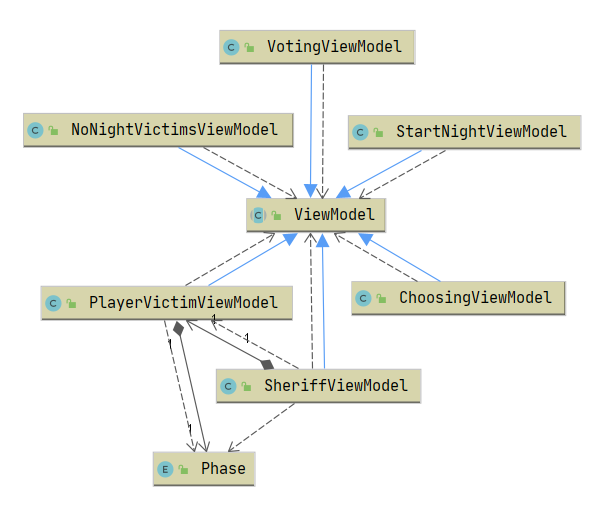
\includegraphics[width=\textwidth]{architektur/View_Uebersicht.png}
	\caption{Übersicht ViewModel (Package)}
	\label{figure:viewmodel(package)}
\end{figure}

Die \autoref{figure:viewmodel(package)} gibt eine grobe Übersicht über die View an. Die Hauptklasse, der View, ist die Klasse \textit{ViewModel}. Die Klasse \textit{VotingViewModel} ermöglicht es den Spielleiter bei einer Wahl zu unterstützen. Um Spieler auszuwählen ist die Klasse \textit{ChoosingViewModel} zuständig. Die Klasse \textit{StartNigthViewModel} wird verwendet für den ersten Start der Nacht, um die richtige nachfolgende Szene zu laden. Das \textit{PlayerVictimViewModel} kann bestimmte Phasen auslösen, wo noch ein weiteres Opfer ausgesucht werden muss oder eine Nachfolge bestimmt werden muss. 
Die Klasse \textit{SheriffViewModel} ist für die Wahl des Hauptmannes zuständig und wenn der Hauptmann stirbt wird, hierüber der Nachfolger bestimmt, welcher vom alten Hauptmann bestimmt wird. Die \textit{NoNightVictimsViewModel} Klasse springt zur nächsten richtigen Szene, die die Hauptmannwahl sein kann oder gleich schon die Lynchabstimmung.

\medskip
Bei der Klasse \textit{ChoosingViewModel} werden wir uns bestimmte Methoden anschauen, welche besonders wichtig sind für den Spielverlauf.
Die \textit{getStart()} Methode markiert für die jeweilige Szene das Liebespaar, welche sich nicht gegenseitig umbringen dürfen.
In der Methode \textit{choosing()} wird die richtige Methode von updateDisplay ausgewählt, für die beiden Szene, welche über das ViewModel angesprochen werden.
Die nextScene Methoden rufen in dem Fall die richtige nachfolgende Szene auf.

\medskip
Die Klasse \textit{VotingViewModel} wird die Abstimmung für das Lynchen am Tag auf gesetzt, welches in der Methode \textit{getStart()} passiert. Die Methoden \textit{nextSceneSheriff...()} sind bei gleichstand vorhandene Actionlistener, welche die Buttons abfragen, welchen der Hauptmann von ihnen umbringen möchte, aber nur wenn ein Hauptmann gewählt wurde. sonst wird in der Methode \textit{getStarted()} eine Stichwahl ausgeführt, mit den Spielern die ein gleichstand haben, außer einer hat mehr.
\textit{reset()} resetet die Comboboxen vom vorherigen Tag und auch die Labels.

\medskip
In der Klasse \textit{SheriffViewModel} wird die Logik für die Wahl des Hauptmannes programmiert. Wenn bei der Wahl ein gleichstand zustande kommt wird nochmals gewählt, wie bei dem \textit{VotingViewModel}, aber wenn es erneut zu einem Gleichstand kommt wird am nächsten Tag erneut gewählt. Diese Klasse hat ein paar extra Methoden und zwar wenn der Hauptmann stirbt, muss er seinen Nachfolger ernennen.

\medskip
Die Klassen \textit{StartNightViewModel} und \textit{NoNightVictimViewModel} sind in teilen identisch, sie unterscheiden sich nur in den aufrufen der nachfolgenden Szenen.

\medskip
Die letzte Klasse in dem Package \textit{PlayerVictimViewModel} behandelt die getöteten Spieler der Runde, damit die der Spielleiter ein Übersicht hat wer alles gestorben ist, um es den Mitspielern mitzuteilen und manche Rollen haben noch eine bestimmte Fähigkeit, wenn sie sterben, welche dann auch abgehandelt wird in der Szene.      

\subsection{ViewModel Board (Package)}

\begin{figure}[H]
	\centering
	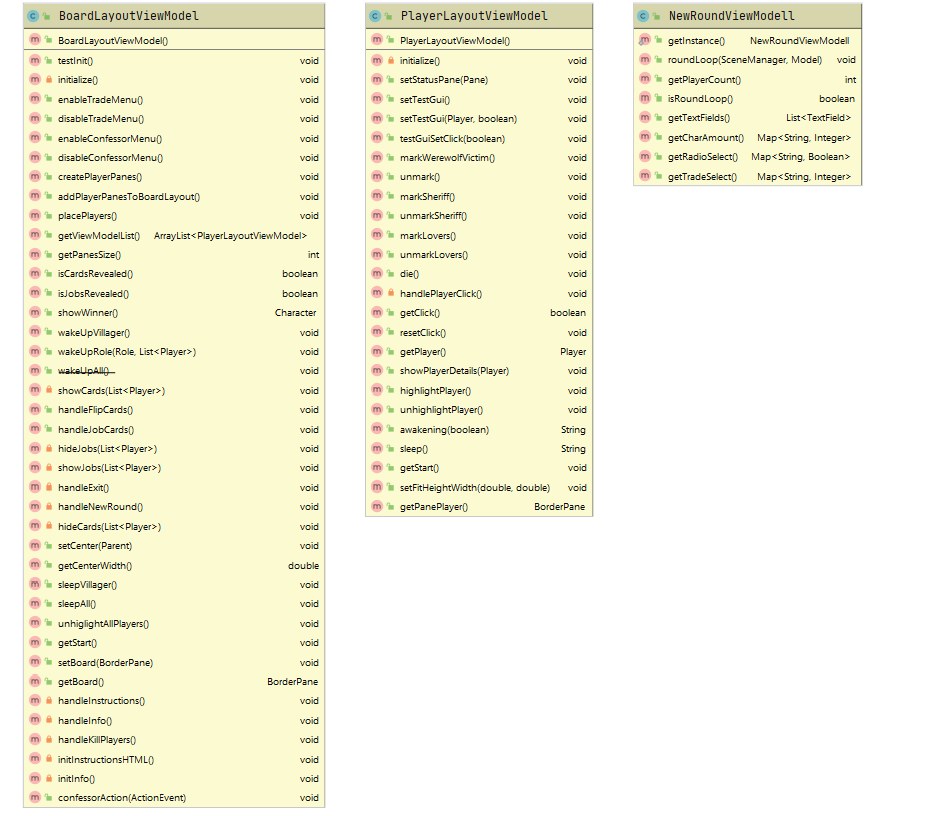
\includegraphics[width=\textwidth]{architektur/View_Board_Uebersicht.png}
	\caption{Übersicht ViewModel Board (Package)}
	\label{figure:viewmodelboard(package)}
\end{figure}

Die Klasse \emph{BoardLayoutViewModel} dient dazu das gesamte Spielfeld anzuzeigen. Auf diesem werden später alle Spieler platziert, sowie alle weiteren Informationen im Laufe des Spiels angezeigt. Dazu basiert das Spielfeld auf einer JavaFX-BorderPane. Die Klasse enthält einige Methoden um Nutzerinteraktionen z.B. über die Menüleiste zu erhalten. Außerdem bietet sie den anderen Programmteilen die Möglichkeit Szenen im Centerfield des BorderPanes anzeigen zu lassen. Weiterhin werden die in der Spielvorbereitung angelegten Spieler entsprechend ihrer Position auf dem Spielfeld platziert. Die maximale mögliche Größe der einzelnen Spielerkarten wird dabei von dieser Klasse errechnet und in den einzelnen Karten festgelegt um in der gegebenen Bildschirmauflösung alle Karten darstellen zu können.

\medskip
Die Klasse \emph{PlayerLayoutViewModel} dient dazu die einzelnen Karten der Spieler auf dem Spielfeld anzuzeigen. Dazu bietet sie Zugriff auf die Elemente der FXML-Datei und setzt hier entsprechend die benötigten CSS-Klassen. Außerdem beinhaltet die Klasse eine Möglichkeit auf Klicks zu reagieren und dabei die Spielerkarte entsprechend zu markieren. Zusätzlich bietet sie die Möglichkeit die Charakterkarte eines Spielers bei seinem Tod in Graustufen darzustellen und sein Statusfeld entsprechend einzufärben. Die Klasse enthält zusätzlich eine Möglichkeit die Größe der Spielerkarte festzulegen.

\medskip
Die Klasse \textit{NewRoundViewModel} wird verwendet wenn der Spielleiter eine Runde zu ende gespielt hat und eine neue Runde anfangen möchte, um das Programm nicht neu zu starten muss. Diese kann der Spielleiter auch während einer laufenden Runde. Es werden alle Information über die Auswahl der Runde gespeichert, welche er in den Szenen zur Gamepreparation anpassen kann.
  

\subsection{ViewModel Character (Package)}

\begin{figure}[H]
	\centering
	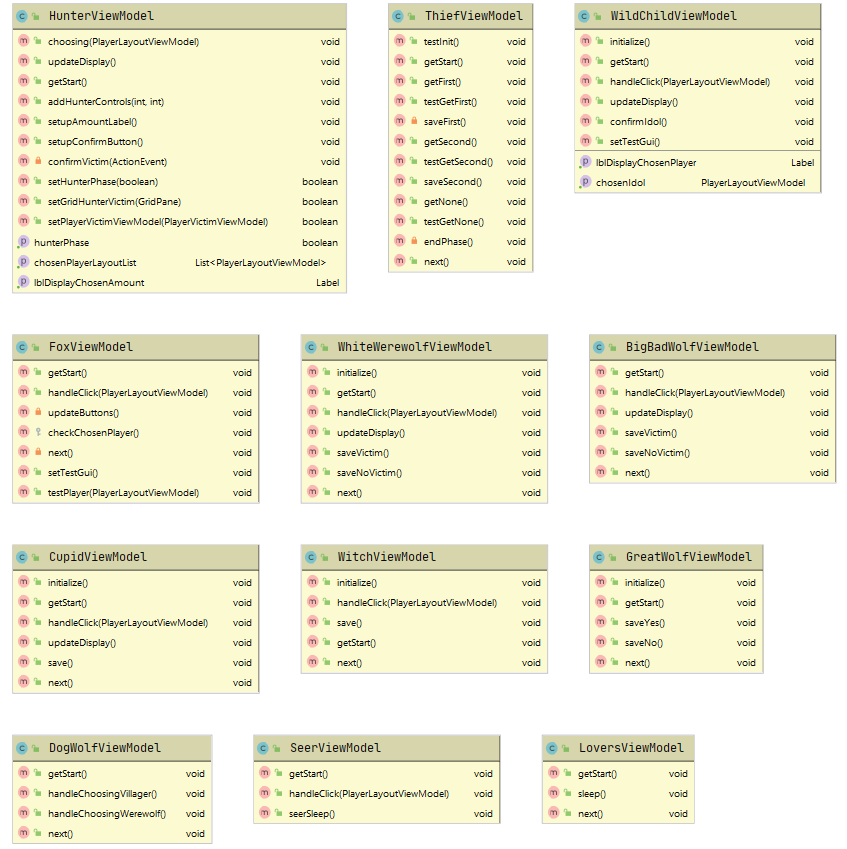
\includegraphics[width=\textwidth]{architektur/View_Char_Uebersicht.png}
	\caption{Übersicht ViewModel Character (Package)}
	\label{figure:viewmodelchar(package)}
\end{figure}

Es wird hier nur auf ein paar Klassen des Package, da die Klassen alle sehr ähnlich Aufgebaut sind.
Die Klassen \textit{SeerViewModel} und \textit{LoversViewModel} sind sehr identisch, sie unterscheiden sich nur in einer Methode, da die Seherin sich pro Nacht eine Karte anschauen kann.

\medskip
Das \textit{ThiefViewModel} merkt sich die Auswahl des Diebes vom Anfang der Spielrunde, um ihn der entsprechenden Fraktion zu zuordnen.

\medskip
Alle Klassen bis auf die \textit{LoversViewModel} haben eine Methode, welche sich um die Auswahl eines anderen Mitspieler kümmert, um die bestimmten Fähigkeiten der Rollen aus zu führen. 

\subsection{ViewModel Gamepreperation (Package)}

\begin{figure}[H]
	\centering
	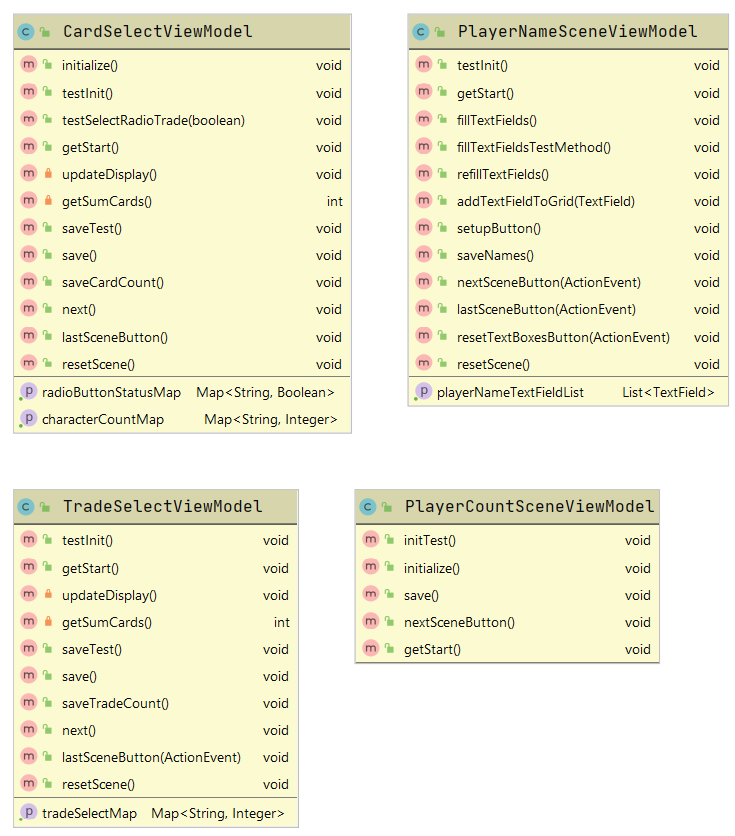
\includegraphics[width=\textwidth]{architektur/View_Game_Uebersicht.png}
	\caption{Übersicht ViewModel Gamepreperation (Package)}
	\label{figure:viewmodelgame(package)}
\end{figure}

Die Klassen in der \autoref{figure:viewmodelgame(package)} zusehen sind, dienen der Voreinstellung für eine Spielrunde getätigt, wenn eine neue Runde über den Loop gestartet wird, werden die Voreinstellungen der Runde zuvor übernommen. Alle Klassen haben die ähnliche Methoden, um die Auswahl zu speichern.
\subsection{ViewModel Trade (Package)}

\begin{figure}[H]
	\centering
	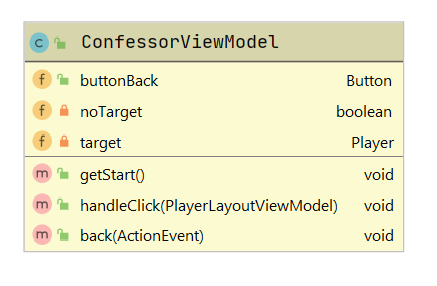
\includegraphics[width=0.6\textwidth]{architektur/View_Trade_Uebersicht.png}
	\caption{Übersicht ViewModel Trade (Package)}
	\label{figure:viewmodeltrade(package)}
\end{figure}

Die Klasse in dem Package behandelt die besondere Funktion des Beichtvaters, welche nur einmal verwendbar ist momentan.

\subsection{SceneManager}

Der \textit{SceneManager} ist die Hauptklasse um die Szenen zu initialisieren und zu laden. Die meisten FXML-Datein werden über die \textit{initFXML()} geladen. Manche Szenen werden über spezielle \textit{init...()} Methoden geladen, da die Szenen Informationen aus vorherigen Szenen benötigen. Die Szenen werden über die \textit{switchToScene()} Methode aufgerufen, über eine switch case wird zwischen den Szenen gewechselt. 

\section{Config}

Der Werwolf-Spielleiter erlaubt dem Benutzer verschiedene Werte der Software über eine JSON Config-Datei anzupassen. Als Beispiel dient hier der Standardwert an Mitspielern welcher beim Start automatisch selektiert wird. Die dazugehörige Config-Datei wird im Wurzelverzeichnis der Software eingelesen oder wenn sie noch nicht existiert, erstellt und mit Standardwerten gefüllt. Die dafür benötigten Klassen werden im Folgenden erläutert.

\subsection{ConfigLoader}

Die \textit{ConfigLoader} Klasse liest alle Konstanten aus der Klasse \textit{PublicGameConstants} aus und fügt diese der \textit{publicGameConstants} Liste hinzu. Mit der Methode \textit{initConfig} wird die Liste mit einer Liste verglichen die der \textit{JSONConfigLoader} aus einer Config-Datei eingelsen hat. Beim Start des Spiels wird an verschiedenen Stellen im Modell die \textit{getOrDefault} Methode aufgerufen. Diese liefert entweder ein Wert den der \textit{JSONConfigLoader} eingelesen hat oder einen Standardwert (Abbildung \ref{lst:configLoader01}).

\medskip
\begin{center}
	\begin{minipage}{0.95\textwidth}
		\lstinputlisting[firstnumber=80, firstline=80, lastline=96, caption=ConfigLoader getOrDefault Methode, label= lst:configLoader01]{../src/main/java/de/werwolf_spielleiter/config/ConfigLoader.java}
	\end{minipage}
\end{center}

\subsection{JSONConfigLoader}

Die \textit{JSONConfigLoader} Klasse wird von der \textit{ConfigLoader} Klasse verwendet um Config-Werte von einem vorgegebenen Pfad aus einer JSON Datei zu lesen. Existiert die Config-Datei unter dem Pfad, dann werden alle ausgelesene Werte dem \textit{ConfigLoader} über den Aufruf der Methode \textit{readConfigFromJSON} übergeben. Existiert die Config-Datei nicht, dann wird eine neue Config-Datei erstellt, welche die Standardwert der \textit{PublicGameConstants} Klasse enthält.

\section{Anspruchsvolle Stellen der Implementierung}

Ein besonders zu Beginn schwieriges Thema war die korrekte Erstellung der FXML-Dateien. Zunächst wurden viele FXML-Dateien separat  angelegt. Durch die vielen Einstellungsmöglichkeiten war es nicht immer ganz einfach, später diverse Einstellungen in csv-Dateien auszulagern. 

\medskip
Ein weiteres Thema war die Initialisierung der FXML-Dateien. Wir haben teilweise einige Anläufe gebraucht, diese korrekt zu initialisieren. Besonders wenn in den Szenen Daten aus dem Spielverlauf benötigt werden, die zu Beginn beim Programmaufruf noch nicht vorhanden sind. Dort wurde aber nach einiger Zeit eine passable Lösung gefunden. 

\medskip
Ein anspruchsvoller Punkt war das Einrichten der Build-Pipeline für JavaFx, da die normale Pipeline um weitere Befehle ergänzt werden musste.
